\documentclass[tikz, border=1pt]{standalone}

\usepackage{xcolor}
\usetikzlibrary{arrows.meta}
\begin{document}
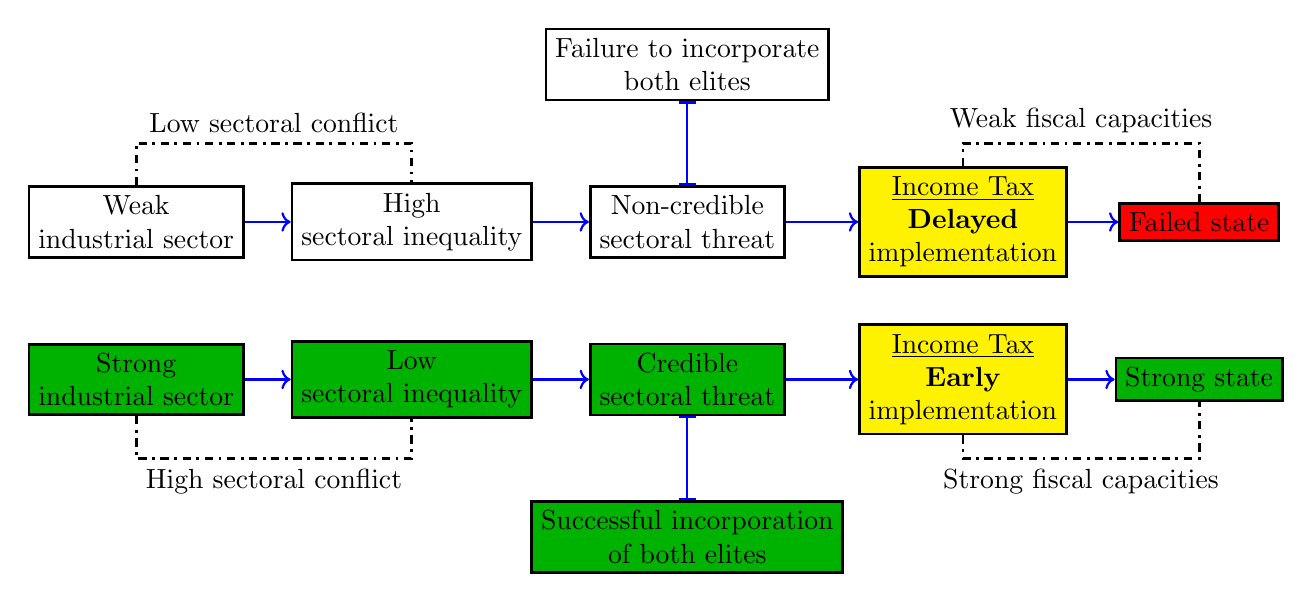
\begin{tikzpicture}[line width=1pt]


% 1
\node[draw,align=center,fill=black!30!green,text=black] (ArgumentA1) at (1,0) {Strong\\industrial sector};
\node[draw,align=center,fill=black!30!green,text=black] (ArgumentB1) at (4.5,0) {Low\\sectoral inequality};
\node[draw,align=center, fill=black!30!green,text=black] (ArgumentC) at (8,0) {Credible\\sectoral threat};
\node[draw,align=center,fill=yellow,text=black] (ArgumentD1) at (11.5,0) {\underline{Income Tax}\\{\bf Early}\\implementation};
\node[draw,align=center,fill=black!30!green,text=black] (ArgumentD3) at (8,-2) {Successful incorporation\\of both elites};
\node[draw,fill=black!30!green,text=black] (ArgumentE1) at (14.5,0) {Strong state};




\draw[->,draw=blue,thick] (ArgumentB1) to (ArgumentC);
\draw[<-,draw=blue,thick] (ArgumentD1) to (ArgumentC);
\draw[->,draw=blue,thick] (ArgumentD1) to (ArgumentE1);
\draw[|-|,draw=blue,thick] (ArgumentC) to (ArgumentD3);
\draw[->,draw=blue,thick] (ArgumentA1) to (ArgumentB1);

\draw[dash dot] (ArgumentA1) -- ++(0,-1) -| (ArgumentB1)
node[below, near start] {High sectoral conflict};

\draw[dash dot] (ArgumentD1) -- ++(0,-1) -| (ArgumentE1)
node[below, near start] {Strong fiscal capacities};


\node at (6., -1.0) {};


% 2
\node[draw,align=center,text=black] (ArgumentA2) at (1,2) {Weak\\industrial sector};
\node[draw,align=center,text=black] (ArgumentB2) at (4.5,2) {High\\sectoral inequality};
\node[draw,align=center] (ArgumentC) at (8,2) {Non-credible\\sectoral threat};
\node[draw,,align=center,fill=yellow,text=black] (ArgumentD2) at (11.5,2) {\underline{Income Tax}\\{\bf Delayed}\\implementation};
\node[draw,align=center] (ArgumentD23) at (8,4) {Failure to incorporate\\both elites};

\node[draw,fill=red,text=black] (ArgumentE2) at (14.5,2) {Failed state};
\draw[->,draw=blue,thick] (ArgumentD2) to (ArgumentE2);
\draw[|-|,draw=blue,thick] (ArgumentC) to (ArgumentD23);




\draw[->,draw=blue,thick] (ArgumentB2) to (ArgumentC);
\draw[<-,draw=blue,thick] (ArgumentD2) to (ArgumentC);
\draw[->,draw=blue,thick] (ArgumentA2) to (ArgumentB2);

\draw[dash dot] (ArgumentA2) -- ++(0,1) -| (ArgumentB2)
node[above, near start] {Low sectoral conflict};

\draw[dash dot] (ArgumentD2) -- ++(0,1) -| (ArgumentE2)
node[above, near start] {Weak fiscal capacities};

\node at (6., -1.0) {};

\end{tikzpicture}
\end{document}